\documentclass[tikz]{standalone}

\usepackage{tikz}
\usetikzlibrary{positioning, arrows.meta}

\begin{document}

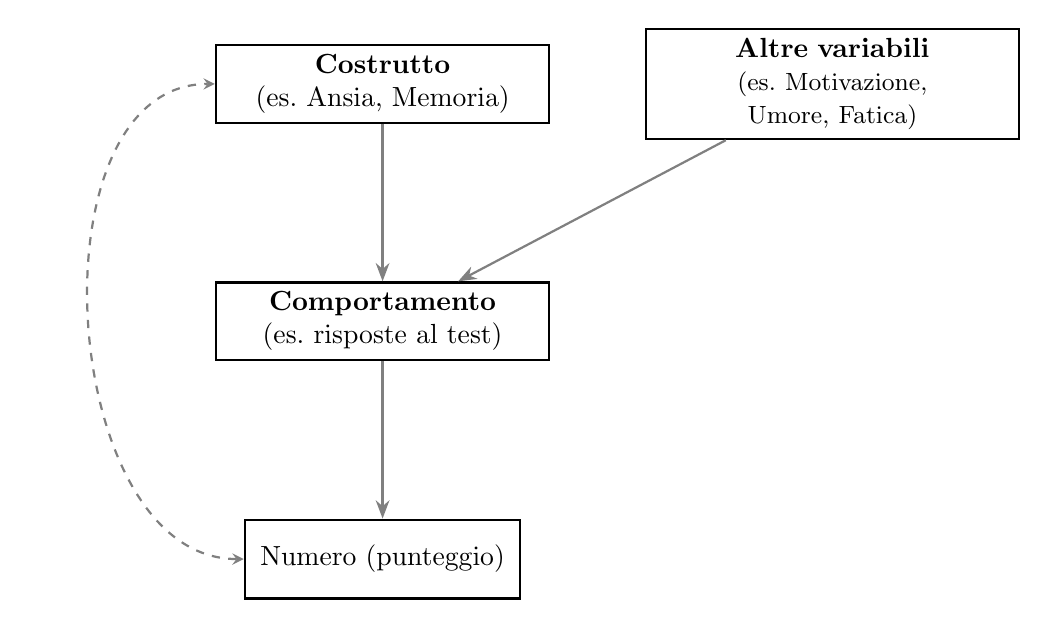
\begin{tikzpicture}[
    node distance=2cm,
    thick
]

\node[draw, rectangle, text width=4cm, align=center] (construct)
    {\textbf{Costrutto} \\ (es.\ Ansia, Memoria)};

\node[draw, rectangle, text width=4cm, align=center, below=2cm of construct] (behaviour)
    {\textbf{Comportamento}\\ (es.\ risposte al test)};

\node[draw, rectangle, minimum width=3.5cm, minimum height=1cm, below=2cm of behaviour] (measure)
    {Numero (punteggio)};

\node[draw, rectangle, text width=4.5cm, align=center, right=1.2cm of construct] (others)
    {\textbf{Altre variabili}\\ {\small(es.\ Motivazione, Umore, Fatica)}};

\draw[-{Stealth}, gray, solid, thick] (construct) -- (behaviour);
\draw[-{Stealth}, gray, solid, thick] (behaviour) -- (measure);
\draw[-{Stealth}, gray, solid, thick] (others) -- (behaviour);
\draw[<->, >=stealth, gray, dashed, thick] (measure) to[out=180, in=180] (construct);

\end{tikzpicture}

\end{document}
